\documentclass[%
    thesis=ma, %
    language=american, %
    paper=a4,%
    listings,
    online,
    %draft,
    final,
]{isw}

%\usepackage{showframe}

\title{This Shall be a Great Thesis Paper with an Extremely Long Title but who Cares because it is just an exemplary title}
\subtitle{Some Theses Even Have Subtitles Which Should Not be as Long as This Subtitle Is Because it is too Long}
\author{Maschinen Bauer}
\major{Mechatronik}
\examiner{Jun.-Prof.~Dr.-Ing.~Andreas Pott}
\supervisor{Dipl.-Ing.~Philipp Tempel \and Dipl.-Ing.~Martin Wehr}
\matriculation{1234567}
\date{2015-08-28}

\usepackage{lipsum}


%% Fill in your thesis' data here
\title{This shall be a great thesis paper with an extremely long title but who cares}
\subtitle{Some theses even have subtitles}
\author{Philipp Tempel}
\major{Technische Kybernetik}
\examiner{Jun.-Prof.~Dr.-Ing.~Andreas Pott}
\major{Technische Kybernetik}
\supervisor{Dipl.-Ing.~Philipp Tempel}
%\matriculation{2411697}

% And done with the configuration you are!

\usepackage{lipsum}

\begin{document}
    \maketitle
    
    \begin{otherlanguage}{ngerman}
        \maketitle
    \end{otherlanguage}
    
    \tableofcontents
    
    \listoffigures
    
    \listoftables
    
    \listoftodos
    
    \chapter[The Short Title of the Chapter Showing Up in the TOC and the Page Headers]{The Very First Chapter With a Very Long Title Just to See What it Looks Like Since it Spans Multiple Lines in the ToC}
    
    \chapter{A Second Chapter}
    
    \section{A First Section}
    
    \subsection{A Sample Subsection}
    
    \subsubsection{A Sample Subsubsection}
    
    \paragraph{A Sample Paragraph}
    
    \subparagraph{A Sample Subparagraph}
    
    \chapter{The Main Template}
    
    \section{Document Structure}
    
    Basically you are free in organizing your document, however, it is recommended that a certain order of chapters is always obeyed to which is
    
    \begin{enumerate}
        \item Table of Contents
        \item List of Figures
        \item List of Tables
        \item List of Abbreviations
        \item List of Symbols (math symbols and alike)
        \item List of Abbreviations (textual abbreviations like e.g., CDPR)
    \end{enumerate}
    
    \begin{figure}
        \centering
        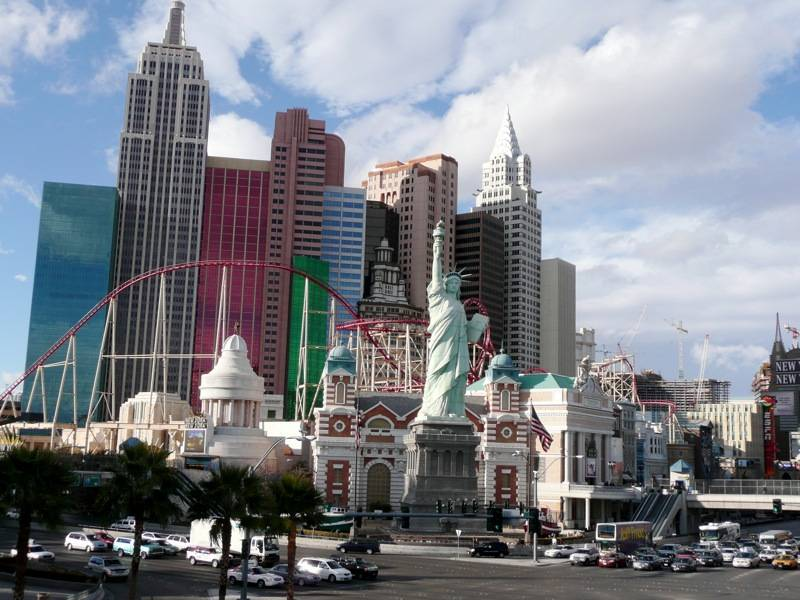
\includegraphics[width=\linewidth, keepaspectratio=true]{placeholder/800-600-1}
        \caption{A sample figure of the New York Hotel at Las Vegas, NV, USA showing the effect of a loooong looooong caption.}
        \label{fig:sample-figure}
    \end{figure}
    
    \begin{figure}
        \centering
        \begin{subfigure}[b]{0.49\textwidth}
            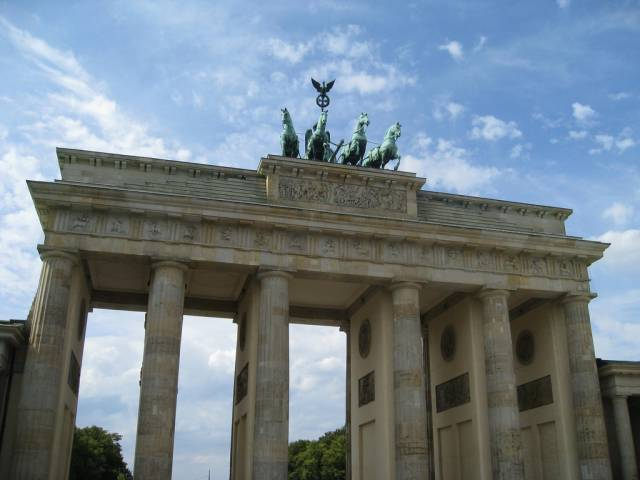
\includegraphics[width=\textwidth, keepaspectratio]{placeholder/640-480-1}
            \caption{Picture 1}
            \label{fig:subfigures-two:1}
        \end{subfigure}
        \hfill
        \begin{subfigure}[b]{0.49\textwidth}
            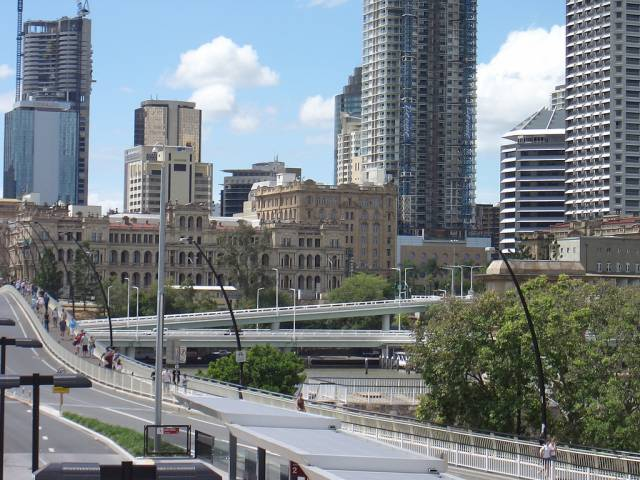
\includegraphics[width=\textwidth, keepaspectratio]{placeholder/640-480-2}
            \caption{Picture 2}
            \label{fig:subfigures-two:2}
        \end{subfigure}
        
        \caption{Even subfigures of two figures are possible}
        \label{fig:subfigures-2}
    \end{figure}
    
    \begin{figure}
        \centering
        \begin{subfigure}[b]{0.49\textwidth}
            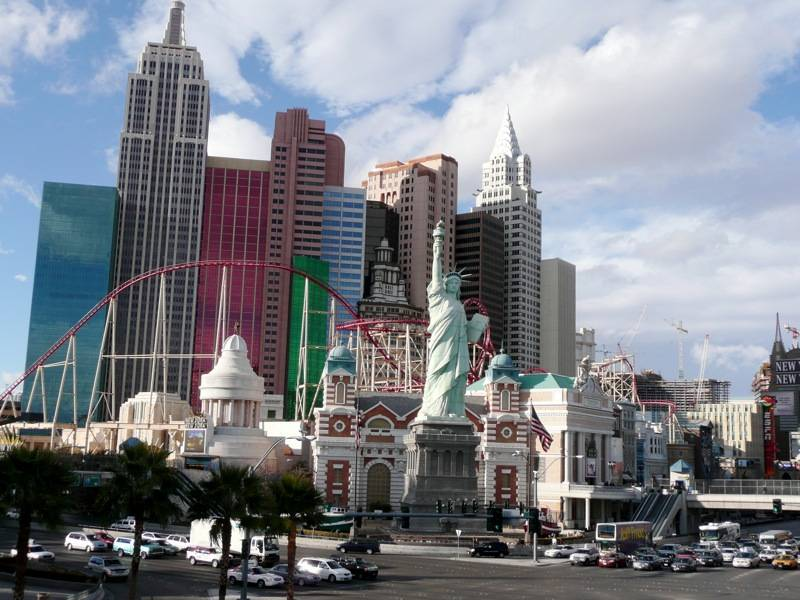
\includegraphics[width=\textwidth, keepaspectratio]{placeholder/800-600-1}
            \caption{Picture 1}
            \label{fig:subfigures-four:1}
        \end{subfigure}
        \hfill
        \begin{subfigure}[b]{0.49\textwidth}
            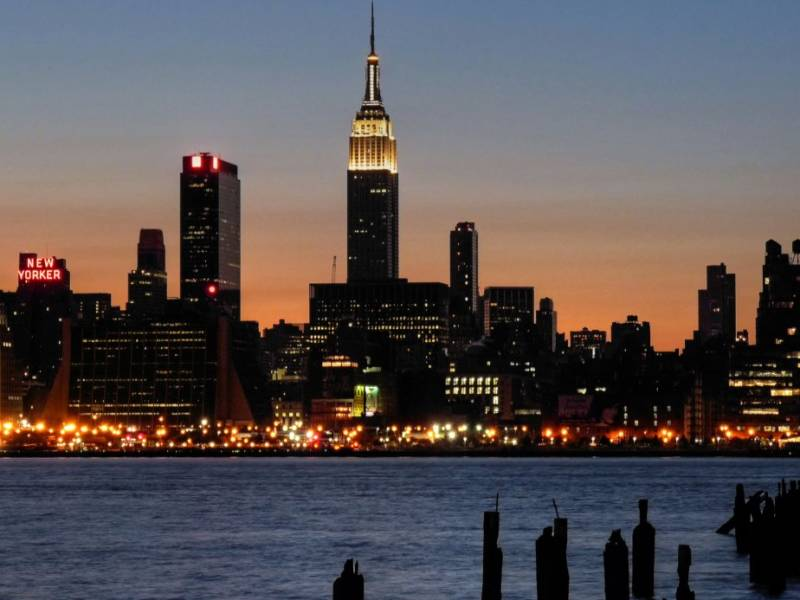
\includegraphics[width=\textwidth, keepaspectratio]{placeholder/800-600-2}
            \caption{Picture 2}
            \label{fig:subfigures-four:2}
        \end{subfigure}
        \hfill
        \begin{subfigure}[b]{0.49\textwidth}
            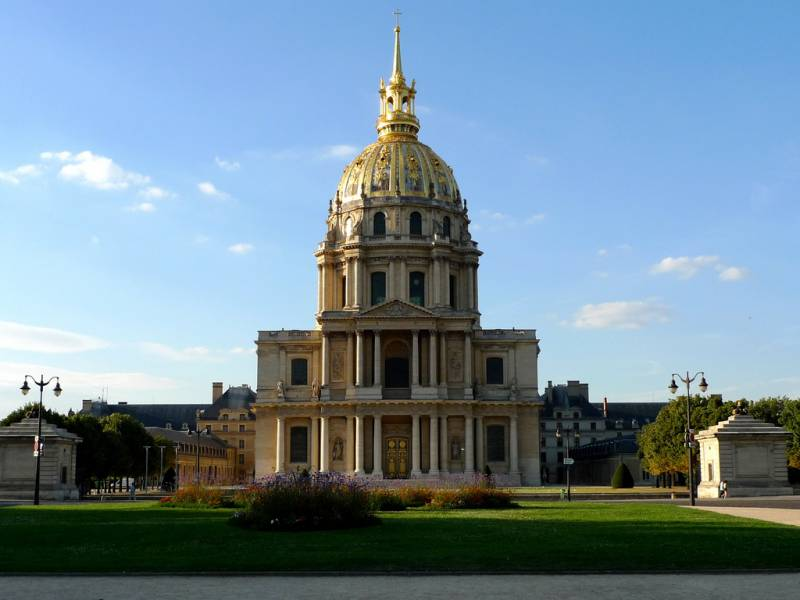
\includegraphics[width=\textwidth, keepaspectratio]{placeholder/800-600-3}
            \caption{Picture 3}
            \label{fig:subfigures-four:3}
        \end{subfigure}
        \hfill
        \begin{subfigure}[b]{0.49\textwidth}
            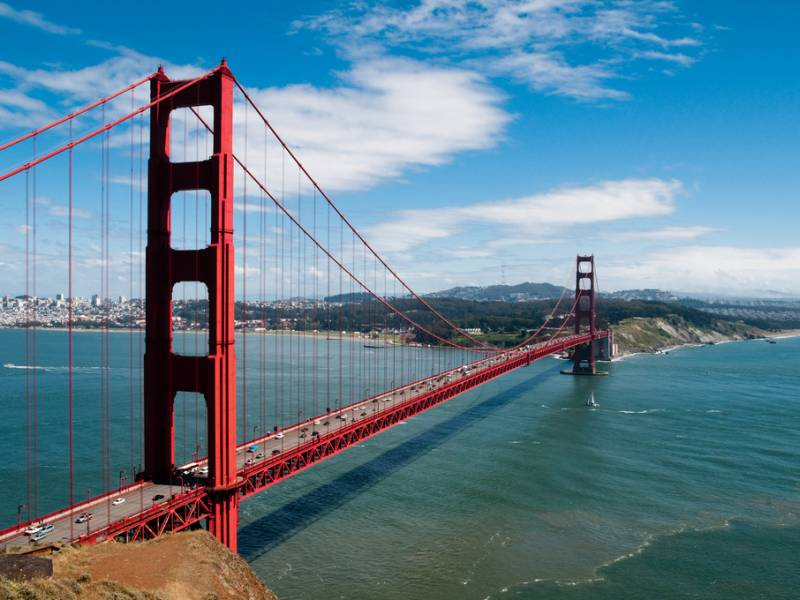
\includegraphics[width=\textwidth, keepaspectratio]{placeholder/800-600-4}
            \caption{Picture 4}
            \label{fig:subfigures-four:4}
        \end{subfigure}
        
        \caption{Even subfigures of four figures are possible}
        \label{fig:subfigures-2}
    \end{figure}
    
    \begin{table}
        \centering
        \caption{A sample table}
        \label{tbl:sample-table}
        \begin{tabular}{@{}llr@{}} \toprule
            \multicolumn{2}{c}{Item} \\ \cmidrule(r){1-2}
            Animal & Description & Price (\$)\\ \midrule
            Gnat  & per gram  & 13.65 \\
            & each      & 0.01 \\
            Gnu   & stuffed   & 92.50 \\
            Emu   & stuffed   & 33.33 \\
            Armadillo & frozen & 8.99 \\ \bottomrule
        \end{tabular}
    \end{table}
    
    \begin{table}
        \centering
        \caption{Tables can look nice, even for many many data to display}
        \label{tbl:sample-table-large}
        \begin{tabular}{SSSSSSSS} \toprule
            {$m$} & {$\Re\{\underline{\mathfrak{X}}(m)\}$} & {$-\Im\{\underline{\mathfrak{X}}(m)\}$} & {$\mathfrak{X}(m)$} & {$\frac{\mathfrak{X}(m)}{23}$} & {$A_m$} & {$\varphi(m)\ /\ ^{\circ}$} & {$\varphi_m\ /\ ^{\circ}$} \\ \midrule
            1  & 16.128 & +8.872 & 16.128 & 1.402 & 1.373 & -146.6 & -137.6 \\
            2  & 3.442  & -2.509 & 3.442  & 0.299 & 0.343 & 133.2  & 152.4  \\
            3  & 1.826  & -0.363 & 1.826  & 0.159 & 0.119 & 168.5  & -161.1 \\
            4  & 0.993  & -0.429 & 0.993  & 0.086 & 0.08  & 25.6   & 90     \\ \midrule
            5  & 1.29   & +0.099 & 1.29   & 0.112 & 0.097 & -175.6 & -114.7 \\
            6  & 0.483  & -0.183 & 0.483  & 0.042 & 0.063 & 22.3   & 122.5  \\
            7  & 0.766  & -0.475 & 0.766  & 0.067 & 0.039 & 141.6  & -122   \\
            8  & 0.624  & +0.365 & 0.624  & 0.054 & 0.04  & -35.7  & 90     \\ \midrule
            9  & 0.641  & -0.466 & 0.641  & 0.056 & 0.045 & 133.3  & -106.3 \\
            10 & 0.45   & +0.421 & 0.45   & 0.039 & 0.034 & -69.4  & 110.9  \\
            11 & 0.598  & -0.597 & 0.598  & 0.052 & 0.025 & 92.3   & -109.3 \\ \bottomrule
        \end{tabular}
    \end{table}
    
%    \begin{lstlisting}
%        \begin{minted}{latex}
%\begin{figure}
%    \centering
%    \includegraphics[width=\linewidth, keepaspectratio=true]%
%        {placeholder/14942249547_f7f1d3e8bd_k}
%    \caption{A sample figure to show the effect of a loooong looooong caption. %
%        Credits by \url{https://www.flickr.com/photos/schubi74/14942249547/}.}
%    \label{fig:sample-figure}
%\end{figure}
%        \end{minted}
%        \caption{Sample code for \cref{fig:sample-figure}}
%        \label{lst:sample-code}
%    \end{lstlisting}
    
    For figures the guidelines are:
    \begin{itemize}
        \item Always center images using \verb|\centering| as the very first command of the \verb|figure|-environment.
        \item Make sure to set the width of your included images explicitely using the \verb|width=\linewidth| option.
        \item Don't forget to keep the aspect ratio of images if you change their width.
        \item Never ever under sample images. In other words: never ever enlarge images.
        \item It's best to use vector graphics i.e., \verb|*.eps| or \verb|*.tikz| for proper quality in both PDFs as well as on screen.
        \item Add a caption to your image. Captions must be below the image.
        \item Let the labels be handled automatically by \LaTeX. A best practice is to set the prefix of figures' labels to \verb|fig:|.
        \item For a good example see \cref{fig:sample-figure} and its code at \cref{lst:sample-code} (this reference was created using the \verb|\cref{}| command).
        \item Always add a full stop to your figure captions like so.
    \end{itemize}
    
    
    \section{Referencing}
    
    Referencing may be done using \verb|\ref{label}| even though usage of \verb|\cref{label}| is encouraged for that it automatically typesets the appropriate type like \texttt{Eqn.} or \texttt{Fig.}, \texttt{Tbl.}, or \texttt{Listing} to whatever is being reference. At the beginning of a sentence \verb|\Cref{label}| must be used to fully the referenced type in words. \Cref{fig:sample-figure} refers to a sample figure at the beginning of a sentence, while \cref{fig:sample-figure} refers to a sample figure in text.
    
    \begin{itemize}
        \item Capitalise and write in words the reference object at the beginning of a sentence
        \item Otherwise use the abbreviated forms of \texttt{Fig.}, \texttt{Eqn.}, and \texttt{Tbl.} for referencing figures, equations, and tables, respectively
        \item Refer to the \verb|cleveref| package documentation at \url {http://www.ctan.org/pkg/cleveref}
    \end{itemize}
    
\end{document}